\documentclass[11pt,a4paper,oneside]{report}

\usepackage{amsmath,amssymb}
\usepackage{parskip}
\usepackage{graphicx}
\usepackage{xcolor}
\usepackage[a4paper,margin=1in]{geometry}
\usepackage{longtable,booktabs,array}

\usepackage{titlesec}
\titleformat{\chapter}[display]
  {\sffamily\bfseries\huge}
  {\Large \chaptertitlename\ \thechapter}
  {2ex}
  {\titlerule
   \vspace{1ex}%
   \filright\MakeUppercase}
  [\vspace{1ex}%
\titlerule]
\titleformat{\section}{\normalfont\sffamily\Large\bfseries}{\thesection}{1em}{}
\titleformat{\subsection}{\normalfont\sffamily\large\bfseries}{\thesubsection}{1em}{}
\titleformat{\subsubsection}{\normalfont\sffamily\normalsize\bfseries}{\thesubsubsection}{1em}{}

\usepackage[style=numeric-comp, url=false]{biblatex}
\addbibresource{bibfile.bib}

\usepackage[no-math]{fontspec}
\usepackage{unicode-math}
\defaultfontfeatures{Ligatures=TeX,Numbers=Lining}
\setmainfont{Source Serif Pro}[BoldFont={Source Serif Pro Semibold}]
\setsansfont{SourceSansPro-Regular}[BoldFont={SourceSansPro-Semibold}]
\IfFontExistsTF{Cambria Math}{\setmathfont{Cambria Math}[Scale=1]}{\setmathfont{Asana Math}}

\usepackage{xeCJK}
\setCJKmainfont{Noto Sans SC}
\setCJKsansfont{Noto Sans SC}

\newcommand{\instructions}[1]{{\color{orange}\itshape #1}}

\usepackage{upquote}
\usepackage[allcolors=blue,colorlinks=true]{hyperref}
\usepackage{xurl}
\usepackage{microtype}
\usepackage{bookmark}
\usepackage{calc}
\usepackage{etoolbox}

\urlstyle{same}

\begin{document}


% Author name (capitalized in its regular way)
\newcommand{\authorname}{Jingheng Huan}

% Title (cannot exceed three lines)
% You can insert manual linebreaks with \\
\newcommand{\thetitle}{A CASE STUDY OF AI IN VISION GENERATION: THE EVOLUTION, APPLICATIONS, AND ETHICS}

% Date of submission with normal capitalization. 
% Use the format January 29, 2022.
\newcommand{\submissiondate}{Mar 7, 2024}

% Mentor: First Name Last Name (normal capitalization)
\newcommand{\mentor}{Peng Sun}

% Academic Unit (no abbreviations)
\newcommand{\academicunit}{Division of Natural and Applied Sciences}

%%%%%%%%%%%%%%%%%%%%%%%%%%%%%%%%%%%%%%%%%%%%%%%%%%%%%%%%%%%%%%%%%%%%%%%%%%%%%%%%

%% DO NOT CHANGE DIRECTLY THE CONTENTS OF THE TITLE PAGE.
%% TO CUSTOMIZE THE TITLE PAGE CHANGE THE DEFINITIONS OF THE COMMANDS
%% \authorname, \thetitle, \submissiondate, \mentor, \academicunit




\begin{titlepage}

\vspace*{\bigskipamount}

\begin{center}
{\sffamily\LARGE\bfseries\MakeUppercase\thetitle\par}

\bigskip

by

\bigskip

{\Large \authorname}

\bigskip

Signature Work Product, in partial fulfillment of the \\
Duke Kunshan University Undergraduate Degree Program

\bigskip

\emph{\submissiondate}

\bigskip

Signature Work Program \\
Duke Kunshan University

\end{center}

\vfill

\textbf{\textsf{APPROVALS}}

\bigskip\bigskip\bigskip
\hrule

Mentor: \mentor, \academicunit

\bigskip\bigskip\bigskip
\hrule

Marcia B. France, Dean of Undergraduate Studies

\end{titlepage}

%%%%%%%%%%%%%%%%%%%%%%%%%%%%%%%%%%%%%%%%%%%%%%%%%%%%%%%%%%%%%%%%%%%%%%%%%%%%%%%%

% Front matter
\clearpage
\pagenumbering{roman}

%%%%%%%%%%%%%%%%%%%%%%%%%%%%%%%%%%%%%%%%%%%%%%%%%%%%%%%%%%%%%%%%%%%%%%%%%%%%%%%%

\setcounter{tocdepth}{0} % Only top-level units (chapters) should appear in the TOC
\tableofcontents

%%%%%%%%%%%%%%%%%%%%%%%%%%%%%%%%%%%%%%%%%%%%%%%%%%%%%%%%%%%%%%%%%%%%%%%%%%%%%%%%

\chapter*{Abstract}
\addcontentsline{toc}{chapter}{Abstract}

% Abstract in English

\instructions{This study delves into the transformative realm of AI-driven generative technologies, 
examining their development and deployment in image and video synthesis. 
Through a comparative analysis of Generative Adversarial Networks (GANs), 
Diffusion Models, and Neural Cellular Automata, the research investigates their underlying theoretical frameworks and experimental applications. 
Key findings reveal nuanced insights into the algorithms' efficacy in generating photorealistic outputs and their potential in various industries. 
The research also critically assesses the ethical landscape, underscoring the importance of safety and fairness in AI-generated content. 
Major conclusions suggest a trajectory towards more autonomous and creative AI systems, while advocating for robust ethical guidelines to govern their use. 
This abstract, a synthesis of the comprehensive document, ensures a precise overview of the research's scope and its major contributions to the field of AI and generative media.}

\vspace{4\bigskipamount}

% Abstract in Chinese

\instructions{本研究深入探讨了人工智能驱动的生成技术的变革领域,研究了这些技术在图像和视频合成中的发展和应用。
通过对生成对抗网络(GANs)、扩散模型和神经细胞自动机的比较分析,研究探讨了它们的基础理论框架和实验应用。
主要发现揭示了这些算法在生成逼真输出方面的功效及其在各行各业的潜力。
研究还对伦理环境进行了批判性评估,强调了人工智能生成内容的安全性和公平性的重要性。
主要结论表明,人工智能系统的发展轨迹将更加自主、更具创造性,同时倡导制定严格的伦理准则来规范人工智能系统的使用。
本摘要是对综合文件的综述,确保准确概述研究范围及其对人工智能和生成式媒体领域的主要贡献。}


%%%%%%%%%%%%%%%%%%%%%%%%%%%%%%%%%%%%%%%%%%%%%%%%%%%%%%%%%%%%%%%%%%%%%%%%%%%%%%%%

\chapter*{Acknowledgements}
\label{acknowledgements}
\addcontentsline{toc}{chapter}{Acknowledgements}

\instructions{Individuals and organizations who helped with the research project
and provided financing are thanked in a paragraph of the thesis. Do not
include individual titles in the acknowledgments. However, it is
appropriate to state grant numbers and sponsors. Examples would like
SELF, SRS, SW Grants, etc.}

\newpage

%%%%%%%%%%%%%%%%%%%%%%%%%%%%%%%%%%%%%%%%%%%%%%%%%%%%%%%%%%%%%%%%%%%%%%%%%%%%%%%%

% Add captions to your figures for them to appear in the List of Figures.
% Alternatively, comment out the next two lines if there are no tables 
% in your document.
\addcontentsline{toc}{chapter}{List of Figures}
\setcounter{tocdepth}{1}
\listoffigures\newpage

%%%%%%%%%%%%%%%%%%%%%%%%%%%%%%%%%%%%%%%%%%%%%%%%%%%%%%%%%%%%%%%%%%%%%%%%%%%%%%%%

% Add captions to your tables for them to appear in the List of Tables.
% Alternatively, comment out the next two lines if there are no tables 
% in your document.
\addcontentsline{toc}{chapter}{List of Tables}
\setcounter{tocdepth}{1}
\listoftables\newpage

%%%%%%%%%%%%%%%%%%%%%%%%%%%%%%%%%%%%%%%%%%%%%%%%%%%%%%%%%%%%%%%%%%%%%%%%%%%%%%%%

% Main matter
\clearpage
\pagenumbering{arabic}

%%%%%%%%%%%%%%%%%%%%%%%%%%%%%%%%%%%%%%%%%%%%%%%%%%%%%%%%%%%%%%%%%%%%%%%%%%%%%%%%

\chapter{Introduction}
\label{introduction}

\instructions{This section includes a clear statement of the problem and the
reasons for studying it.~Provide a detailed yet concise background
discussion of the problem and the significance, scope, and limits of the
work. Outline what has been done previously by citing truly pertinent
literature but do not include a general survey of semi-relevant
literature.~ State how your work differs from earlier work in the field
and demonstrate the continuity from the previous work to your own.}

%%%%%%%%%%%%%%%%%%%%%%%%%%%%%%%%%%%%%%%%%%%%%%%%%%%%%%%%%%%%%%%%%%%%%%%%%%%%%%%%

\chapter{Material and Methods}
\label{material-and-methods}

\instructions{The workflow of this video-creating project is shown below:

1: Write the storyline of the video, including plots, storyboards, 
2: Collect and edit the video footage.
3: Use AI-generated content to create the visuals.
4: Edit the visuals to create the desired effect.
5: Post-production to clean up the video and add music and sound effects.
6: Publish the video on social media and other platforms.

This section should include a detailed description of the materials and
methods used in the project. It should include the equipment, techniques,
and procedures used to create the video. It is important to include
details such as the software used, the hardware used, and the process
used to create the video. It is also important to describe the
constraints and limitations of the project, such as the time and
resources available to complete the project. Finally, it is important
to describe the ethical considerations of the project, such as the
potential for bias and discrimination in the content generated by the
AI-generated content.
}

%%%%%%%%%%%%%%%%%%%%%%%%%%%%%%%%%%%%%%%%%%%%%%%%%%%%%%%%%%%%%%%%%%%%%%%%%%%%%%%%

\chapter{Results}
\label{results}

\instructions{Summarize the data collected in this section, and their
statistical treatment. Include only relevant data, but give sufficient
detail to justify the conclusions. It is appropriate in this section to
use equations, figures, and tables to display your data. Extensive, but
relevant data, should be reserved for an appendix where it is identified
as supporting information.}

\instructions{The table or figure must follow as closely as possible after the
paragraph in which it is referenced. Titles/captions should be kept
brief.}

\section{Examples}

Here is some inline math, $x^2 > 1$, and some display math
\begin{equation}
  \int_0^1 x^2 \, dx
\end{equation}
And this is how to cite an article \cite{Zhang2021} or a book \cite{Axler2020}.

\begin{table}[htbp]
\centering
\begin{tabular}{@{}llll@{}}
\toprule
\emph{Replace} & \emph{With} & \emph{Your} & \emph{Table} \\
\midrule
& & & \\
& & & \\
\bottomrule
\end{tabular}
\caption{Parameters for the optimization of the principal component analysis for
olive oil adulteration.}
\label{tbl:2}  
\end{table}


\begin{figure}[htbp]
\centering
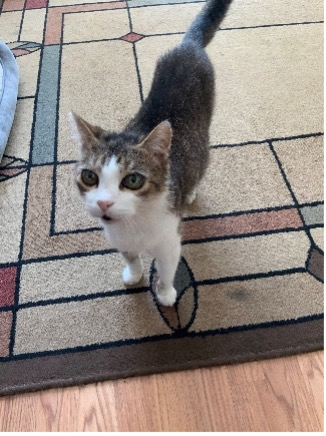
\includegraphics[height=4cm]{btc.jpg}
\caption{The notorious BTC (Brandon The Cat).}
\label{fig:1}
\end{figure}

%%%%%%%%%%%%%%%%%%%%%%%%%%%%%%%%%%%%%%%%%%%%%%%%%%%%%%%%%%%%%%%%%%%%%%%%%%%%%%%%

\chapter{Discussion}
\label{discussion}

\instructions{The discussion section is where you interpret and compare the
results. The objective is to point out the features and limitations of
the work. Relate your results to current knowledge in the field and to
the original purpose for undertaking the project.}

%%%%%%%%%%%%%%%%%%%%%%%%%%%%%%%%%%%%%%%%%%%%%%%%%%%%%%%%%%%%%%%%%%%%%%%%%%%%%%%%

\chapter{Conclusions}
\label{conclusions}

\instructions{This section is written to put the interpretation of the results
into the context of the original problem.~ Do not repeat the discussion
points or include irrelevant material. The conclusion should be based on
the evidence presented.}

%%%%%%%%%%%%%%%%%%%%%%%%%%%%%%%%%%%%%%%%%%%%%%%%%%%%%%%%%%%%%%%%%%%%%%%%%%%%%%%%

\chapter*{References}
\label{references}
\addcontentsline{toc}{chapter}{References}


\instructions{Many bibliographic styles are acceptable for publications 
in the natural sciences. This template uses a numeric style defined in biblatex
and that is common in Physics, Mathematics, and Computer Science papers.}

\printbibliography[heading=none]

%%%%%%%%%%%%%%%%%%%%%%%%%%%%%%%%%%%%%%%%%%%%%%%%%%%%%%%%%%%%%%%%%%%%%%%%%%%%%%%%

\appendix

\chapter{Additional Material}
\label{appendix-a}

This template can be viewed on Overleaf at \url{https://www.overleaf.com/read/hxjcgtkhjqcd}.
If you have an Overleaf account (either free or paid) you can copy this template to start a new Overleaf project.
If you do not want an Overleaf account you can install TeX on your computer and download the template files from Overleaf.

\end{document}